\chapter{Dérivés des acides carboxyliques}\label{ch:b2:acyl-substitution}

Faire bouillir de l'huile d'olive avec de la soude donne du savon et du glycérol~: c'est la plus
ancienne réaction organique menée à dessein. L'huile est un ester du glycérol et d'acides à
longue chaîne, et l'hydroxyde coupe chaque ester au niveau d'une liaison, toujours la même, entre
le carbone du carbonyle et l'oxygène de l'alcool. Esters, acides, amides, anhydrides et \omterm{def:b2:acyl-substitution:derivative}{chlorures
d'acyle} réagissent tous de cette façon~: un nucléophile s'additionne sur le carbone du carbonyle,
et un groupe part. Classer ces composés selon l'aptitude de leur groupe à partir indique lesquels
peuvent être transformés en lesquels, et dans quel sens un chimiste doit remonter la pente.

\begin{recall}
Le volume de première année~: activation électrophile d'un groupe carbonyle, mécanismes de
formation des hémiacétals et des acétals, additions d'organomagnésiens, donneurs d'hydrure et leur
portée, groupes partants, $\mathrm pK_a$, $Q$ et $K$. \Cref{ch:b2:amines}~: \omterm{def:b2:amines:nucleophilic-addition}{addition
nucléophile}, amines. \Cref{ch:b2:equilibrium-shifts}~: déplacer un équilibre. Le volume scolaire~:
esters, acides carboxyliques et amides.
\end{recall}

\begin{omfigure}
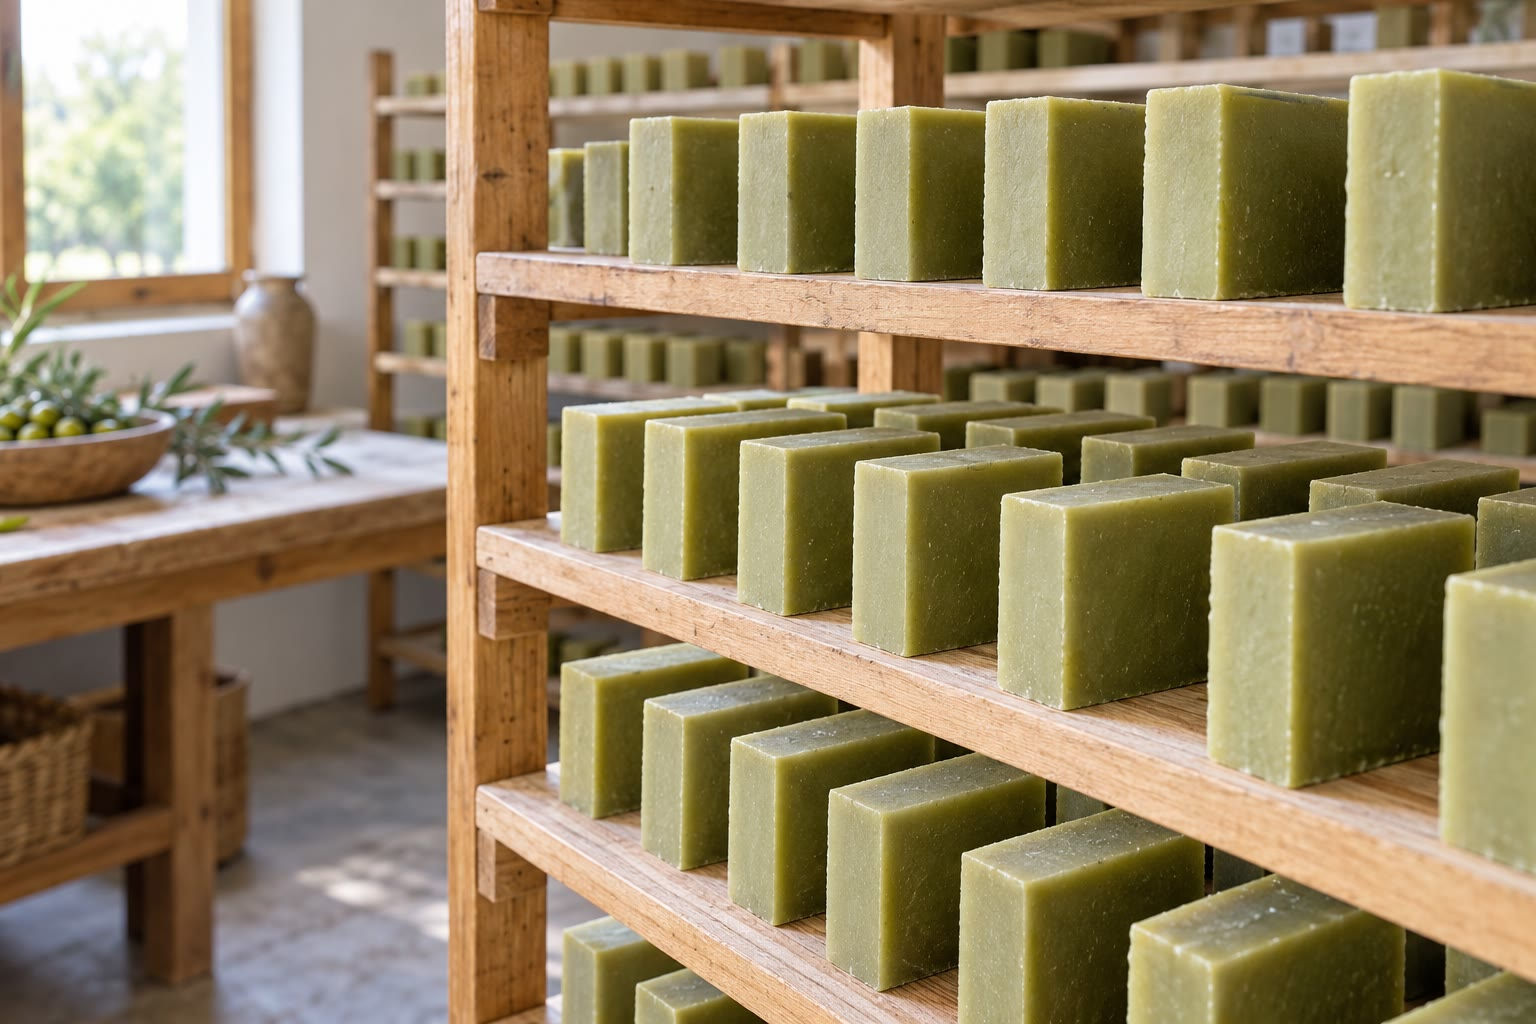
\includegraphics[width=0.58\linewidth]{images/book3/ai/b2-24-soap-bars.jpg}

{\small Pains de savon à l'huile d'olive séchant sur des claies en bois. Le savon est le sel de
sodium des acides gras libérés quand on fait bouillir l'huile, un ester, avec de la soude.}
\end{omfigure}

\section{La famille et sa réactivité}

\begin{definition}[Dérivés des acides carboxyliques]\label{def:b2:acyl-substitution:derivative}
Un \emph{dérivé d'acide carboxylique}\index{derive d'acide carboxylique@dérivé d'acide carboxylique} est un composé \ce{R-CO-Z}
dans lequel le \ce{OH} d'un acide carboxylique est remplacé par un autre groupe Z. Le \emph{groupe
acyle}\index{groupe acyle} $\mathrm{R{-}CO{-}}$ leur est commun à tous. Dans un \emph{chlorure d'acyle}\index{chlorure d'acyle},
Z est Cl~; dans un \emph{anhydride d'acide}\index{anhydride d'acide}, Z est $\mathrm{O{-}CO{-}R'}$, deux groupes
acyle partageant un même oxygène~; dans un ester, Z est $\mathrm{OR'}$, dans un amide $\mathrm{NR'_2}$.
\end{definition}

\begin{proposition}[Échelle de réactivité]\label{prop:b2:acyl-substitution:reactivity}
Vis-à-vis des nucléophiles, les dérivés réagissent dans l'ordre \omterm{def:b2:acyl-substitution:derivative}{chlorure d'acyle} $>$ anhydride $>$
ester $\approx$ acide $>$ amide.
\end{proposition}

\begin{proof}[Argument]
Deux effets s'ajoutent. Le groupe partant \ce{Z-} part d'autant plus facilement que c'est une base
plus faible~: \ce{Cl-} (acide conjugué \ce{HCl}, $\mathrm pK_a$ vers $-7$) bien mieux qu'un
carboxylate ($\mathrm pK_a$ vers 5), un alcoolate (vers 16) ou un ion amidure (vers 35). Et le
groupe Z cède de la densité électronique au carbonyle par effet mésomère donneur de son doublet, ce
qui rend le carbone du carbonyle moins électrophile~: faiblement pour Cl, le plus fortement pour
l'azote. L'amide est à la fois le moins bon électrophile et le moins bon groupe partant.
% ledger: pka:ethanoic, pka:ethanol
\end{proof}

\section{Substitution nucléophile acyle}

\begin{definition}[Substitution nucléophile acyle]\label{def:b2:acyl-substitution:nas}
Une \emph{substitution nucléophile acyle}\index{substitution nucleophile acyle@substitution nucléophile acyle} remplace le groupe Z
d'un composé acylé par un nucléophile. Elle procède par addition du nucléophile sur le carbone du
carbonyle, qui donne un \emph{intermédiaire tétraédrique}\index{intermediaire tetraedrique@intermédiaire tétraédrique}, suivie de
l'élimination du groupe partant, qui reforme la liaison \ce{C=O}.
\end{definition}

\begin{proposition}[Addition--élimination]\label{prop:b2:acyl-substitution:addition-elimination}
La substitution acyle passe par un \omterm{def:b2:acyl-substitution:nas}{intermédiaire tétraédrique}~; elle est accélérée en milieu
basique par un nucléophile plus fort et en milieu acide par l'activation du carbonyle.
\end{proposition}

\begin{proof}[Argument]
Le carbone du carbonyle, plan et électrophile, reçoit le nucléophile par-dessus ou par-dessous son
plan, comme dans les additions du \cref{ch:b2:amines}~; avec un groupe Z capable de partir,
l'intermédiaire l'expulse au lieu d'être protoné. En milieu basique, le nucléophile est un anion
(\ce{HO-}, \ce{RO-})~; en milieu acide, l'oxygène du carbonyle est protoné et un nucléophile neutre
(l'eau, un alcool) suffit. Des esters marqués à l'\ce{^{18}O} dans leur partie alcool donnent, par
hydrolyse, un alcool marqué et un acide non marqué~: la liaison rompue est la liaison acyle--oxygène,
comme l'exige le mécanisme.
\end{proof}

\begin{omfigure}
\setchemfig{atom sep=1.7em}
\schemestart
\chemfig{R-C(=[2]O)-OR'} \+ \chemfig{HO^{-}}
\arrow{->[addition]}
\chemfig{R-C(-[2]O^{-})(-[6]OH)-OR'}
\arrow{->[élimination]}[,1.3]
\chemfig{R-C(=[2]O)-OH} \+ \chemfig{^{-}OR'}
\schemestop

\medskip
\schemestart
\chemfig{R-C(=[2]O)-OH} \+ \chemfig{^{-}OR'}
\arrow{->[transfert de proton]}
\chemfig{R-C(=[2]O)-O^{-}} \+ \chemfig{HOR'}
\schemestop
\par\vspace{6pt}

{\small \omterm{def:b2:acyl-substitution:saponification}{Saponification} d'un ester. L'hydroxyde s'additionne sur le carbone du carbonyle, ce qui
donne l'\omterm{def:b2:acyl-substitution:nas}{intermédiaire tétraédrique}~; l'alcoolate part et la liaison \ce{C=O} se reforme~;
l'alcoolate, base forte, arrache ensuite le proton de l'acide. Cette dernière étape rend la réaction totale.}
\end{omfigure}

\begin{method}[Écrire une substitution acyle]\label{met:b2:acyl-substitution:nas-mechanism}
\begin{enumerate}
  \item En milieu basique~: le nucléophile anionique s'additionne sur le carbone du carbonyle~; la
        charge négative passe sur l'oxygène~; la liaison \ce{C=O} se reforme et Z part~; terminer
        par l'éventuelle étape acide--base.
  \item En milieu acide~: protoner l'oxygène du carbonyle~; le nucléophile neutre s'additionne~;
        transférer un proton au groupe partant~; celui-ci part sous forme de molécule neutre~;
        déprotoner le carbonyle.
  \item Compter les étapes~: chaque intermédiaire est soit tétraédrique, soit un composé carbonylé.
\end{enumerate}
\end{method}

\section{Esters}

\begin{definition}[Estérification]\label{def:b2:acyl-substitution:esterification}
Une \emph{estérification}\index{esterification@estérification} forme un ester à partir d'un acide carboxylique (ou d'un
dérivé plus réactif) et d'un alcool. La réaction directe d'un acide avec un alcool, catalysée par
un acide fort, est l'estérification de Fischer.
\end{definition}

\begin{proposition}[Estérification de Fischer]\label{prop:b2:acyl-substitution:fischer}
L'\omterm{def:b2:acyl-substitution:esterification}{estérification} de Fischer est un équilibre lent, de constante voisine de 4 pour les alcools
primaires~; on la déplace par un excès de l'un des réactifs ou en éliminant l'eau au fur et à
mesure de sa formation.
\end{proposition}

\begin{proof}[Argument]
L'éthanol et l'acide éthanoïque en quantités équimolaires s'arrêtent quand les deux tiers de l'acide sont estérifiés~: $K =
(2/3)^2/(1/3)^2 = 4$. Avec $Q < K$ maintenu par un excès d'alcool, ou en distillant l'eau
(l'appareil de Dean--Stark du volume de première année), la réaction avance davantage
(\cref{ch:b2:equilibrium-shifts}). Les six étapes du mécanisme sont celles de la \cref{met:b2:acyl-substitution:nas-mechanism}
en milieu acide, toutes renversables.
% ledger: ester:berthelot
\end{proof}

\begin{definition}[Saponification]\label{def:b2:acyl-substitution:saponification}
Une \emph{saponification}\index{saponification} est l'hydrolyse d'un ester par un hydroxyde, qui
donne le sel de carboxylate et l'alcool.
\end{definition}

\begin{proposition}[La saponification est totale]\label{prop:b2:acyl-substitution:saponification}
La \omterm{def:b2:acyl-substitution:saponification}{saponification} est totale~: sa dernière étape, le transfert de proton de l'acide carboxylique à
l'alcoolate, a une constante d'équilibre de l'ordre de $10^{11}$.
\end{proposition}

\begin{proof}
Pour $\mathrm{RCOOH + R'O^- \to RCOO^- + R'OH}$,
\[
  K = \frac{K_a(\ce{RCOOH})}{K_a(\mathrm{R'OH})} = 10^{\mathrm pK_a(\mathrm{R'OH}) - \mathrm pK_a(\ce{RCOOH})} ;
\]
avec l'acide éthanoïque (4.76) et l'éthanol (15.93), $K = 10^{11.2}$. Le carboxylate, mauvais électrophile, n'est pas attaqué par l'alcool~: la réaction
globale ne revient pas en arrière.
% ledger: pka:ethanoic, pka:ethanol
\end{proof}

\begin{omfigure}
\setchemfig{atom sep=1.7em}
\schemestart
\chemfig{CH_2(-[0]O-CO-R)-[6]CH(-[0]O-CO-R)-[6]CH_2-[0]O-CO-R}
\+ \chemfig{3\,NaOH}
\arrow{->[chauffage]}
\chemfig{CH_2(-[0]OH)-[6]CH(-[0]OH)-[6]CH_2-[0]OH}
\+ \chemfig{3\,R-COO^{-}\,Na^{+}}
\schemestop
\par\vspace{6pt}

{\small \omterm{def:b2:acyl-substitution:saponification}{Saponification} d'un triglycéride~: les trois liaisons ester sont coupées, ce qui donne le
glycérol et trois molécules du carboxylate de sodium, le savon (R une longue chaîne, \ce{C17H33}
pour l'oléate de l'huile d'olive).}
\end{omfigure}

\begin{definition}[Transestérification]\label{def:b2:acyl-substitution:transesterification}
Une \emph{transestérification}\index{transesterification@transestérification} échange la partie alcool d'un ester,
$\mathrm{RCOOR' + R''OH \rightleftharpoons RCOOR'' + R'OH}$, par catalyse acide ou basique.
\end{definition}

\begin{definition}[Lactones et lactames]\label{def:b2:acyl-substitution:lactone}
Une \emph{lactone}\index{lactone} est un ester cyclique, formé par \omterm{def:b2:acyl-substitution:esterification}{estérification} interne d'un
hydroxyacide~; un \emph{lactame}\index{lactame} est un amide cyclique.
\end{definition}

\section{Dérivés activés}

Descendre l'échelle de réactivité est facile~: un \omterm{def:b2:acyl-substitution:derivative}{chlorure d'acyle} donne un anhydride, un ester ou
un amide avec le nucléophile adéquat, souvent à température ambiante. Remonter exige une
activation~: un acide carboxylique est transformé en chlorure par le chlorure de thionyle,
\[
  \ce{RCOOH + SOCl2 -> RCOCl + SO2 + HCl} ,
\]
dont les sous-produits sont gazeux. Le \omterm{def:b2:acyl-substitution:derivative}{chlorure d'acyle} réagit ensuite avec un alcool ou une
amine~; une base (pyridine, triéthylamine, ou un second équivalent de l'amine) piège le \ce{HCl}
formé, qui protonerait sinon l'amine.

\begin{method}[Passer d'un dérivé à l'autre]\label{met:b2:acyl-substitution:ladder}
\begin{enumerate}
  \item Pour descendre l'échelle (chlorure $\to$ anhydride $\to$ ester, acide $\to$ amide)~: traiter
        par le nucléophile, avec une base pour capter l'acide libéré.
  \item Pour remonter l'échelle~: transformer d'abord l'acide en chlorure (\ce{SOCl2})~; un ester ou
        un amide est d'abord hydrolysé en acide.
  \item Entre un acide et un ester~: \omterm{def:b2:acyl-substitution:esterification}{estérification} de Fischer (équilibre) ou \omterm{def:b2:acyl-substitution:saponification}{saponification}
        (totale) suivie d'une acidification.
\end{enumerate}
\end{method}

\begin{omfigure}
\begin{tikzpicture}[font=\small, >={Stealth}]
  \foreach \y/\n in {4/{chlorure d'acyle \ce{RCOCl}}, 3/{anhydride \ce{(RCO)2O}}, 2/{ester $\mathrm{RCOOR'}$ \quad acide \ce{RCOOH}}, 1/{amide $\mathrm{RCONR'_2}$}} {
    \node[cyclenode, minimum width=5.2cm] at (0,\y*1.1) {\n};
  }
  \draw[->, thick, omDef] (-3.1,4.3) -- (-3.1,1.1) node[midway, left, align=right, font=\scriptsize] {facile~:\\ nucléophile\\ + base};
  \draw[->, thick, omThm] (3.1,2.2) -- (3.1,4.4) node[midway, right, align=left, font=\scriptsize] {en montée~:\\ par l'acide\\ et \ce{SOCl2}};
  \node[font=\scriptsize, anchor=south] at (0,4.85) {plus réactif};
  \node[font=\scriptsize, anchor=north] at (0,0.55) {moins réactif};
\end{tikzpicture}

{\small L'échelle de réactivité des dérivés des acides carboxyliques. Tout dérivé peut être
transformé par un nucléophile en un dérivé situé plus bas~; pour monter, on passe par l'acide et
son chlorure.}
\end{omfigure}

\section{Organométalliques et hydrures}

\begin{proposition}[Deux additions de Grignard]\label{prop:b2:acyl-substitution:grignard-ester}
Un ester traité par un excès d'organomagnésien donne un alcool tertiaire portant deux groupes
identiques venant du réactif.
\end{proposition}

\begin{proof}[Argument]
La première addition donne un \omterm{def:b2:acyl-substitution:nas}{intermédiaire tétraédrique} qui expulse l'alcoolate~: une cétone.
Une cétone est plus électrophile qu'un ester (pas d'effet mésomère donneur d'un groupe $\mathrm{OR'}$)
et réagit avec le réactif plus vite que l'ester restant~; la seconde addition, sur la cétone, donne
l'alcoolate d'un alcool tertiaire, que l'hydrolyse acide finale protone. On ne peut pas arrêter la
réaction à la cétone.
\end{proof}

\begin{proposition}[Réductions par les hydrures]\label{prop:b2:acyl-substitution:hydrides}
L'aluminohydrure de lithium réduit les esters et les acides en alcools primaires, et les amides en
amines~; le borohydrure de sodium réduit les aldéhydes et les cétones mais pas les esters, les
acides ni les amides. Un hydrure d'aluminium encombré (DIBAL-H) à \qty{-78}{\degreeCelsius} réduit
un ester en aldéhyde.
\end{proposition}

\begin{proof}[Argument]
\ce{LiAlH4} est un donneur d'hydrure fort~: comme le réactif de Grignard, il s'additionne deux fois
sur un ester (en passant par l'aldéhyde). Le borohydrure est trop faible pour le carbonyle d'ester,
moins électrophile. Avec le DIBAL-H à basse température, l'\omterm{def:b2:acyl-substitution:nas}{intermédiaire tétraédrique}, retenu par
l'aluminium, n'expulse l'alcoolate qu'à l'hydrolyse aqueuse, quand il ne reste plus d'hydrure~:
l'aldéhyde survit. Dans un amide, c'est l'oxygène, lié à l'aluminium, qui est éliminé au lieu de
l'azote, ce qui laisse un ion iminium que l'hydrure réduit en amine.
\end{proof}

\begin{history}[Chevreul et les corps gras]
\begin{minipage}[t]{0.22\linewidth}
\vspace{0pt}
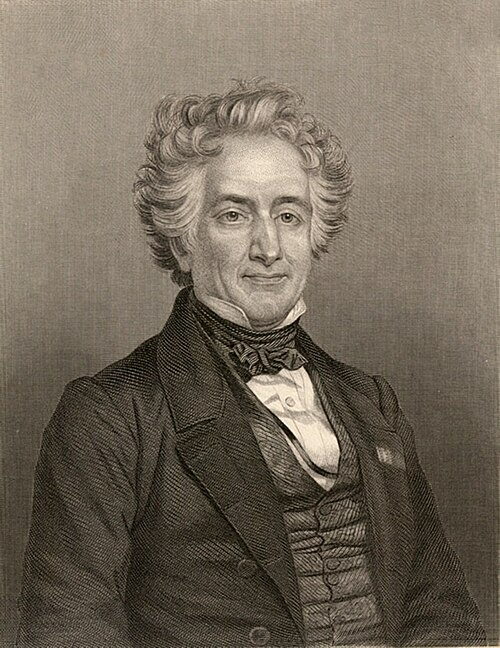
\includegraphics[width=\linewidth]{images/book3/chevreul.jpg}
\end{minipage}\hfill
\begin{minipage}[t]{0.74\linewidth}
\vspace{0pt}
Michel Eugène Chevreul montra, dans une étude publiée en 1823, que les corps gras sont des
combinaisons du glycérol avec des acides gras, qu'il isola et nomma (acides stéarique, oléique,
butyrique), et que la \omterm{def:b2:acyl-substitution:saponification}{saponification} les scinde en ces deux parties. Ses travaux firent de la
fabrication des savons et des bougies une affaire de chimie~; il vécut jusqu'à 102 ans. (Portrait
par Nicolas Eustache Maurin, domaine public, Wikimedia Commons.)
\end{minipage}
\end{history}

\begin{safety}{\ghs[5mm]{GHS02}\,\ghs[5mm]{GHS05}\,\ghs[5mm]{GHS06}}
Le chlorure de thionyle et les \omterm{def:b2:acyl-substitution:derivative}{chlorures d'acyle} réagissent violemment avec l'eau et libèrent des
gaz corrosifs~; on les manipule à sec, sous hotte. L'aluminohydrure de lithium s'enflamme au
contact de l'eau~; son excès est détruit avec précaution à la fin. La soude concentrée est
corrosive pour la peau et les yeux. Le méthanol est toxique et inflammable.
% ledger: ghs:SOCl2, ghs:ethanoyl-chloride, ghs:LiAlH4, ghs:NaOH, ghs:methanol
\end{safety}

\section{Exercices}

\begin{exercise}[$\star$]\label{exo:b2:acyl-substitution:1}
Classer par réactivité vis-à-vis de l'eau~: l'éthanoate d'éthyle, le chlorure d'éthanoyle,
l'éthanamide, l'anhydride éthanoïque.
\end{exercise}

\begin{exercise}[$\star$]\label{exo:b2:acyl-substitution:2}
Donner les produits du chlorure d'éthanoyle avec~: l'eau~; l'éthanol~; l'ammoniac (2 équivalents)~;
l'éthanoate de sodium~; la diméthylamine en présence de triéthylamine.
\end{exercise}

\begin{exercise}[$\star$]\label{exo:b2:acyl-substitution:3}
Écrire la \omterm{def:b2:acyl-substitution:saponification}{saponification} du benzoate de méthyle par la soude et calculer la masse d'hydroxyde de
sodium nécessaire pour \qty{13.6}{g} d'ester.
\end{exercise}

\begin{exercise}[$\star$]\label{exo:b2:acyl-substitution:4}
Représenter la \omterm{def:b2:acyl-substitution:lactone}{lactone} formée par l'acide 4-hydroxybutanoïque et donner la taille de son cycle.
\end{exercise}

\begin{exercise}[$\star\star$]\label{exo:b2:acyl-substitution:5}
Écrire le mécanisme de la réaction de l'éthanoate d'éthyle avec l'ammoniac.
\end{exercise}

\begin{exercise}[$\star\star$]\label{exo:b2:acyl-substitution:6}
L'aspirine est préparée à partir de l'acide salicylique (acide 2-hydroxybenzoïque) et de l'anhydride
éthanoïque. Quel groupe de l'acide salicylique réagit, et quel est le sous-produit~?
\end{exercise}

\begin{exercise}[$\star\star$]\label{exo:b2:acyl-substitution:7}
L'éthanoate d'éthyle est traité par un excès de bromure de méthylmagnésium, puis par un acide dilué.
Donner le produit et expliquer pourquoi la cétone ne peut pas être isolée.
\end{exercise}

\begin{exercise}[$\star\star$]\label{exo:b2:acyl-substitution:8}
Donner le produit de la réduction de la \omterm{def:b2:acyl-substitution:lactone}{lactone} de l'exercice 4 par \ce{LiAlH4}.
\end{exercise}

\begin{exercise}[$\star\star$]\label{exo:b2:acyl-substitution:9}
Avec $K = 4$, calculer la fraction d'acide éthanoïque estérifiée avec un, puis avec trois
équivalents d'éthanol. Quelle autre méthode permet de déplacer la réaction~?
\end{exercise}

\begin{exercise}[$\star\star\star$]\label{exo:b2:acyl-substitution:10}
Préparer le \textit{N},\textit{N}-diéthylbenzamide à partir de l'acide benzoïque, et expliquer
pourquoi mélanger l'acide avec la diéthylamine et chauffer modérément donne plutôt un sel.
\end{exercise}

\begin{exercise}[$\star\star\star$]\label{exo:b2:acyl-substitution:11}
L'indice de \omterm{def:b2:acyl-substitution:saponification}{saponification} d'un corps gras est la masse d'hydroxyde de potassium, en mg, nécessaire
pour saponifier \qty{1}{g} de ce corps gras. Le calculer pour la trioléine (\qty{885.4}{g/mol}~; KOH \qty{56.11}{g/mol}).
\end{exercise}

\begin{exercise}[$\star\star\star$]\label{exo:b2:acyl-substitution:12}
Une molécule porte un ester, un amide et une cétone. Quel(s) groupe(s) \ce{NaBH4} réduit-il, et
lesquels \ce{LiAlH4}~? Qu'obtient-on dans chaque cas~?
\end{exercise}

\section{Problème~: du biodiesel à partir d'huile de friture}

\begin{problem}[{Problème du week-end --- la trioléine et sa masse molaire, sa transestérification
par le méthanol et le rôle de la base, la réaction parasite avec les acides libres et l'eau, et les
rendements par tonne d'huile}]
\label{pb:b2:acyl-substitution:1}
Modéliser l'huile par de la trioléine pure, le triglycéride de l'acide oléique (\ce{C17H33COOH}).
Masses molaires (\unit{g/mol})~: C 12.011, H 1.008, O 15.999, Na 22.990. Le glycérol est le propane-1,2,3-triol.
% ledger: aw:C, aw:H, aw:O, aw:Na, ghs:methanol, ghs:NaOH

\medskip
\noindent\textbf{Partie I --- La trioléine.}
\begin{enumerate}
  \item Donner la formule de l'acide oléique et celle du glycérol.
  \item Écrire la formule de la trioléine et calculer sa masse molaire.
  \item Combien contient-elle de groupes ester~?
  \item L'acide oléique possède une double liaison cis. Pourquoi les huiles qui en sont riches sont-elles liquides à température ambiante~?
  \item Que donnerait la \omterm{def:b2:acyl-substitution:saponification}{saponification} de la trioléine~?
  \item Qu'est-ce que le biodiesel, du point de vue chimique~?
\end{enumerate}

\medskip
\noindent\textbf{Partie II --- \omterm{def:b2:acyl-substitution:transesterification}{Transestérification}.}
\begin{enumerate}[resume]
  \item Écrire la \omterm{def:b2:acyl-substitution:transesterification}{transestérification} de la trioléine par le méthanol.
  \item Pourquoi utilise-t-on une base (méthanolate ou hydroxyde de sodium) comme catalyseur~?
  \item Représenter l'\omterm{def:b2:acyl-substitution:nas}{intermédiaire tétraédrique} du premier échange.
  \item Pourquoi le méthanol est-il utilisé en excès (six équivalents plutôt que trois)~?
  \item Le glycérol n'est pas miscible aux esters méthyliques. En quoi cela aide-t-il~?
  \item Le catalyseur est-il consommé dans la réaction idéale~?
\end{enumerate}

\medskip
\noindent\textbf{Partie III --- Acides libres et eau.}
\begin{enumerate}[resume]
  \item L'huile de friture usagée contient de l'acide oléique libre. Quel est son effet sur la base~?
  \item Quel est l'effet de l'eau sur les esters méthyliques en présence de la base~?
  \item Pourquoi le savon formé est-il gênant~?
  \item Comment éliminer d'abord les acides libres, sans base~?
  \item Pourquoi faut-il sécher l'huile avant la réaction~?
\end{enumerate}

\medskip
\noindent\textbf{Partie IV --- Par tonne d'huile.}
\begin{enumerate}[resume]
  \item Calculer la quantité de trioléine dans une tonne.
  \item Calculer la masse de méthanol consommée.
  \item Calculer la masse d'oléate de méthyle formée.
  \item Vérifier la conservation de la masse.
  \item Une huile contenant 2~\% en masse d'acide oléique libre est traitée par l'hydroxyde de sodium~:
        calculer la masse d'hydroxyde de sodium consommée par l'acide, par tonne.
  \item Calculer la masse de glycérol coproduite par tonne de trioléine.
\end{enumerate}
\end{problem}
